\documentclass[12pt]{article}
\usepackage{graphicx} % This lets you include figures
\usepackage{hyperref} % This lets you make links to web locations
\graphicspath{ {./images/} }

\usepackage[rightcaption]{sidecap}
\usepackage{caption}
\usepackage{subcaption}
\usepackage{hyperref}

\usepackage{float}

\usepackage{imakeidx}

\usepackage{amsmath}
\usepackage{latexsym}
\usepackage{wasysym}


\makeindex


\title{Exercises on LTL}
\author{Beau De Clercq}
\date{October 2019}

\begin{document}
\maketitle{}

%\tableofcontents

\clearpage
\newpage

\section*{Ex. 3.1}
\subsection*{Question}
Give the traces on the set of atomic propositions $\{a,b\}$ of the following transition
system:\\
\begin{centering}
	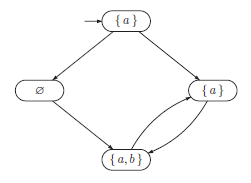
\includegraphics[]{ex31.PNG}
\end{centering}

\subsection*{Answer}

\newpage

\section*{Ex. 3.2}
\subsection*{Question}
On page 97, a transformation is described of a transition system $TS$ with possible
terminal states into an ´´equivalent'' transition system $TS^*$ without terminal states. Questions:
\begin{itemize}
	\item Give a formal definition of this transformation $TS \mapsto TS^*$.
	\item Prove that the transformation preserves trace-equivalence, i.e., show that if $TS_1$, $TS_2$ are
	transition systems (possibly with terminal states) such that Traces($TS_1$) = Traces($TS_2$),
	then Traces($TS^*_1$) = Traces($TS^*_2$).
\end{itemize}

\subsection*{Answer}

\newpage

\section*{Ex. 3.5}
\subsection*{Question}
Consider the set AP of atomic propositions defined by AP = $\{x = 0, x > 1\}$
and consider a nonterminating sequential computer program P that manipulates the variable x.\\
Formulate the following informally stated properties as LT properties:
\begin{itemize}
	\item false
	\item initially x is equal to zero
	\item initially x differs from zero
	\item initially x is equal to zero, but at some point x exceeds one
	\item x exceeds one only finitely many times
	\item x exceeds one infinitely often
	\item the value of x alternates between zero and two
	\item true
\end{itemize}

\subsection*{Answer}

\newpage

\section*{Ex. 3.6}
\subsection*{Question}
Consider the set AP = $\{A,B\}$ of atomic propositions. Formulate the following
properties as LT properties and characterize each of them as being either an invariance, safety
property, or liveness property, or none of these.
\begin{itemize}
	\item A should never occur,
	\item A should occur exactly once,
	\item A and B alternate infinitely often,
	\item A should eventually be followed by B.
\end{itemize}

\subsection*{Answer}

\newpage

\section*{Ex. 3.7}
\subsection*{Question}
Consider the following sequential hardware circuit:\\
\begin{centering}
	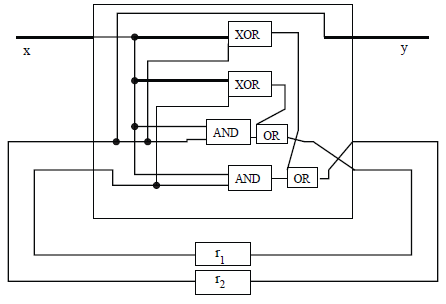
\includegraphics[]{ex37.PNG}
\end{centering}\\
The circuit has input variable $x$, output variable $y$, and registers $r_1$ and $r_2$ with initial values
$r_1$ = 0 and $r_2$ = 1. The set AP of atomic propositions equals $\{ x, r_1, r_2, y \}$. Besides, consider the
following informally formulated LT properties over AP:\\
P1 : Whenever the input $x$ is continuously high (i.e., $x$=1), then the output $y$ is infinitely often
high.\\
P2 : Whenever currently $r_2=0$, then it will never be the case that after the next input, $r_1=1$.\\
P3 : It is never the case that two successive outputs are high.\\
P4 : The configuration with $x=1$ and $r_1=0$ never occurs.\\
\begin{itemize}
	\item Give for each of these properties an example of an infinite word that belongs to $P_i$. Do the
	same for the property $(2^{AP})^\omega \backslash P_i $, i.e., the complement of $P_i$.
	\item Determine which properties are satisfied by the hardware circuit that is given above.
	\item Determine which of the properties are safety properties. Indicate which properties are invariants.
	\begin{itemize}
		\item For each safety property $P_i$, determine the (regular) language of bad prefixes.
		\item For each invariant, provide the propositional logic formula that specifies the property
		that should be fulfilled by each state.
	\end{itemize}
\end{itemize}

\subsection*{Answer}

\newpage

\section*{Ex. 3.8}
\subsection*{Question}
Let LT properties $P$ and $P'$ be equivalent, notation $P \cong P'$, if and only if
pref($P$) = pref($P'$). Prove or disprove: $P \cong P'$ if and only if closure($P$) = closure($P'$).

\subsection*{Answer}


\section*{Ex. 3.9}
\subsection*{Question}
Show that for any transition system $TS$, the set closure(Traces($TS$)) is a safety
property such that $TS \models $ closure(Traces($TS$)).

\subsection*{Answer}

\newpage
\section*{Ex. 3.10}
\subsection*{Question}
Let P be an LT property. Prove: pref(closure(P)) = pref(P).

\subsection*{Answer}

\section*{Ex. 3.11}
\subsection*{Question}
Let $P$ and $P'$ be liveness properties over AP. Prove or disprove the following
claims:
\begin{itemize}
	\item $P \cup P'$ is a liveness property,
	\item $P \cap P'$ is a liveness property.
\end{itemize}
Answer the same question for $P$ and $P'$ being safety properties.

\subsection*{Answer}

\end{document}